\documentclass{article} % For LaTeX2e
\usepackage{nips14submit_e,times}
\usepackage{amsmath}
\usepackage{amsthm}
\usepackage{amssymb}
\usepackage{mathtools}
\usepackage{hyperref}
\usepackage{url}
\usepackage{algorithm}
\usepackage[noend]{algpseudocode}
%\documentstyle[nips14submit_09,times,art10]{article} % For LaTeX 2.09

\usepackage{mathrsfs}
\usepackage{graphicx}
\usepackage{caption}
\usepackage{subcaption}

\def\eQb#1\eQe{\begin{eqnarray*}#1\end{eqnarray*}}
\def\eQnb#1\eQne{\begin{eqnarray}#1\end{eqnarray}}
\providecommand{\e}[1]{\ensuremath{\times 10^{#1}}}
\providecommand{\pb}[0]{\pagebreak}


\def\Qb#1\Qe{\begin{question}#1\end{question}}
\def\Sb#1\Se{\begin{solution}#1\end{solution}}

\newenvironment{claim}[1]{\par\noindent\underline{Claim:}\space#1}{}
\newtheoremstyle{quest}{\topsep}{\topsep}{}{}{\bfseries}{}{ }{\thmname{#1}\thmnote{ #3}.}
\theoremstyle{quest}
\newtheorem*{definition}{Definition}
\newtheorem*{theorem}{Theorem}
\newtheorem*{lemma}{Lemma}
\newtheorem*{question}{Question}
\newtheorem*{preposition}{Preposition}
\newtheorem*{exercise}{Exercise}
\newtheorem*{challengeproblem}{Challenge Problem}
\newtheorem*{solution}{Solution}
\newtheorem*{remark}{Remark}
\usepackage{verbatimbox}
\usepackage{listings}

\title{Real Variables: \\
Problem Set XII}


\author{
Youngduck Choi \\
Courant Institute of Mathematical Sciences \\
New York University \\
\texttt{yc1104@nyu.edu} \\
}


% The \author macro works with any number of authors. There are two commands
% used to separate the names and addresses of multiple authors: \And and \AND.
%
% Using \And between authors leaves it to \LaTeX{} to determine where to break
% the lines. Using \AND forces a linebreak at that point. So, if \LaTeX{}
% puts 3 of 4 authors names on the first line, and the last on the second
% line, try using \AND instead of \And before the third author name.

\newcommand{\fix}{\marginpar{FIX}}
\newcommand{\new}{\marginpar{NEW}}

\nipsfinalcopy % Uncomment for camera-ready version

\begin{document}


\maketitle

\begin{abstract}
This work contains solutions to the problem set 
XII of Real Variables 2015 at NYU.
\end{abstract}

\section{Solutions}

\begin{question}[1. Royden 7-10]
\hfill
\begin{figure}[h!]
  \centering
    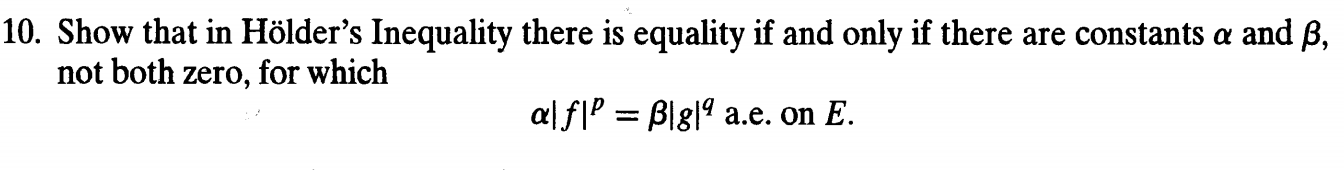
\includegraphics[width=1\textwidth]{7-10.png}
\end{figure}
\end{question}
\begin{solution}

\end{solution}

\newpage

\begin{question}[2. Royden 7-26]
\hfill
\begin{figure}[h!]
  \centering
    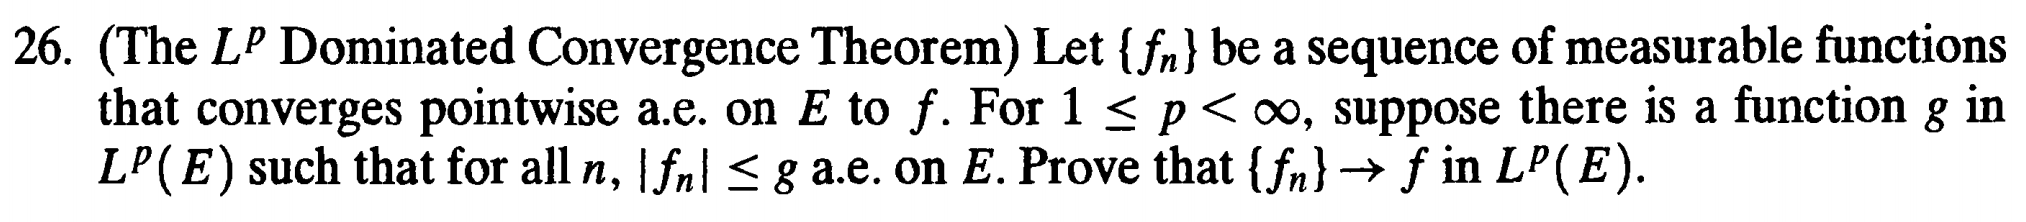
\includegraphics[width=1\textwidth]{7-26.png}
\end{figure}
\end{question}
\begin{solution}
First, we denote the set at which $\{f_n \}$ converges to $f$ pointwise
as $E_0$. 
Then, notice that for any $x \in E_0$ such that $|f_n(x)| \leq g(x)$, 
by the linearity of limit, and the continuity of absolute value,
 we obtain that $|f(x)| \leq g(x)$.
Hence,
we see that $|f| \leq g$ on $E_0$. It follows that
\eQb
|f - f_n| &\leq& |f| + |f_n| \\
&\leq& 2g,
\eQe
on $E_0$. Raising both sides by $p$, we obtain
\eQb
|f - f_n|^p &\leq& 2^p g^p, 
\eQe 
on $E_0$. As sum and product of measurable functions is measurable, 
$\{ f - f_n\}$ is a sequence of measurable functions that converge to
$0$ pointwise, and dominated by $2^p g^p$ everywhere on $E_0$. 
As $g \in L^{P}(E)$, we have that $2^p g^p$ is integrable. With 
the fact that $m(E\setminus E_0) = 0$, by
the Lebesque dominated convergence theorem, we have 
\eQb
\lim_{n \to \infty} \int_{E} |f - f_n|^p &=&
\lim_{n \to \infty} \int_{E_0} |f - f_n|^p \\ 
&=& \int_{E_0} 0 \\
&=& 0.
\eQe 
Hence, $\{ f_n\}$ is convergent to $f$ in $L^P(E)$.
\hfill $\qed$ 
 
\end{solution}

\newpage

\begin{question}[3. Royden 19-5]
\hfill
\begin{figure}[h!]
  \centering
    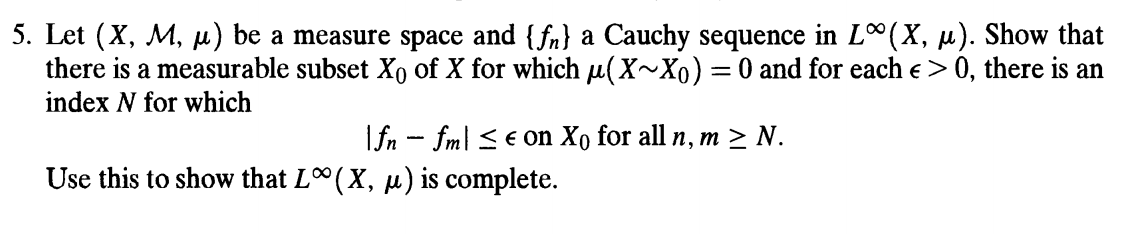
\includegraphics[width=1\textwidth]{19-5.png}
\end{figure}
\end{question}
\begin{solution}
Let $\{ f_k \}$ be a Cauchy sequence in $L^{\infty}(X,u)$. Hence, there
exists $k_n$ such that $|| f_i - f_j ||_{\infty} < \dfrac{1}{n}$ for
$i,j \geq k_n$. 
\end{solution}

\newpage

\begin{question}[4. Royden 17-19]
\hfill
\begin{figure}[h!]
  \centering
    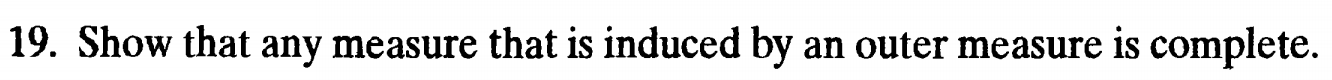
\includegraphics[width=1\textwidth]{17-19.png}
\end{figure}
\end{question}
\begin{solution}
Let $u^*:2^X \to [0,\infty]$ be an outer-measure, and let
$(X,\mathscr{M},u)$ be a measure space induced by $u^*$. Let $E \in 
\mathscr{M}$ and $u(E) = 0$. Let $S \subseteq E$, and $A \in \mathscr{M}$.
Then, by finite monotonicity of $u^*$, we have $u^*(S) = 0$ and $u^*(S 
\cap A) = 0$. Again, using the finite 
monotonicity of $u^*$, we see that
\eQb
u^*(A) &\geq& u^*(A \cap S^c) + 0 \\
&=& u^*(A \cap S^c) + u^*(A \cap S).
\eQe 
Hence, $S \in \mathscr{M}$. We have shown that $u$ is complete.
 \hfill $\qed$
\end{solution}

\newpage

\begin{question}[5. Royden 17-29]
\hfill
\begin{figure}[h!]
  \centering
    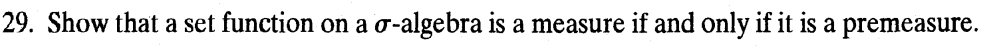
\includegraphics[width=1\textwidth]{17-29.png}
\end{figure}
\end{question}
\begin{solution}
Let $(X,\mathscr{M})$ be a measurable space. Let $u:\mathscr{M} \to 
[0,\infty]$ be a measure. By definition of measure we have, $u(\emptyset)
= 0$. $u$ is finitely additive and countably monotone, 
as any measure has finite additivity and countable monotonicity properties.
Conversely, assume that $u$ is a pre-measure. As $u$ is a pre-measure and 
$\emptyset \in \mathscr{M})$, we have $u(\emptyset) = 0$. Now, let 
$\{E_k \}_{k=1}^{\infty}$ be a countable disjoint collections chosen from
$\mathscr{M}$. By finite additivity, and 
countable monotonicity of $u$, it follows that
\eQb
\sum_{k=1}^{n} u(E_k) &=& u(\bigcup_{k=1}^{n} E_k) \\ 
&\leq& u(\bigcup_{k=1}^{\infty} E_k), \\
\eQe
for all $n$. Hence, by linearity of limits, we obtain
\eQb
\sum_{k=1}^{\infty} u(E_k) &\leq& 
u(\bigcup_{k=1}^{\infty} E_k).
\eQe 
By finite additivity of $u$ and the fact that
 $u(E_k) \geq 0$ for all $k$, we have 
\eQb
\sum_{k=1}^{\infty} u(E_k) &\geq& \sum_{k=1}^{n} u(E_k) \\
&=& u(\bigcup_{k=1}^{n} E_k),
\eQe
for all $n$. Again, by linearity of limits, we obtain that
\eQb
\sum_{k=1}^{\infty} u(E_k) &\geq& u(\bigcup_{k=1}^{\infty}E_k). 
\eQe 
Therefore, we have shown that 
\eQb
\sum_{k=1}^{\infty} u(E_k) &=& u(\bigcup_{k=1}^{\infty}E_k), 
\eQe 
which shows that $u$ is countably additive. Hence, $u$ is a measure.
The claim is true.
\hfill $\qed$

 
\end{solution}

\newpage

\begin{question}[6. Royden 17-36]
\hfill
\begin{figure}[h!]
  \centering
    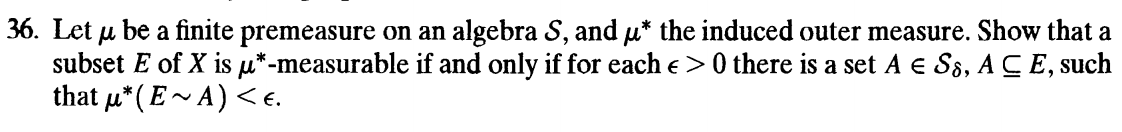
\includegraphics[width=1\textwidth]{17-36.png}
\end{figure}
\end{question}
\begin{solution}
By the definition of set measurability by Caretheodory, $E$ being
$u^*$ measurable is equivalent to $E^c$ being $u^*$ measurable. From Royden,
we have that $E$ is $u^*$ measurable iff for any $\epsilon > 0$,
there exists $A \in S_{\sigma}$ 
such that $A \subseteq S_{\sigma}$, and $u^{*}(A \setminus C) < \epsilon $.

\smallskip
 
We begin the main part of the proof.
Assume $E$ is $u^*$ measurable. Fix $\epsilon > 0$.
Then, by the established equivalence above,
it follows that $E^c$ is $u^*$ measurable, and there exists $A \in S_{\sigma}$
such that $E^c \subseteq A$, and $u^{*}(A \setminus E^c) < \epsilon $.
We claim that $A^c$ is the set with the desired property. As $A \in S_{\sigma}$
there exists $\{ O_n \}_{n=1}^{\infty}$ such that $A = \cup_{n=1}^{\infty}
O_n$. By DeMorgan's law, we have $A^c = \cap_{n=1}^{\infty} {O_n}^{c}$. As,
$S$ is an algebra, ${O_n}^c$ is also in $S$, and it follows that $A^c \in 
S_{\delta}$. Furthermore, as $E^c \subseteq A$, it follows that $A^c \subseteq
E$. Lastly, as $A \setminus E^c = E \setminus A^c$, we have $u^{*}(
E \setminus A^c) < \epsilon$. Since $\epsilon$ was arbitrary, we have shown
the forward implication. 

Now, we prove the reverse implication. Assume that $E$ from $2^X$ has the
given property.  
Fix $\epsilon > 0$. Then, there exists $A \in S_{\delta}$ such that $A \subseteq
E$, and $u^{*}(E\setminus A) < \epsilon$. Then, by taking the argument
above in reverse, we obtain that $A^c \in S_{\sigma}$ such that 
$E^c \subseteq A^c$ and $u^{*}(A^c \setminus E^c) < \epsilon$. Since $\epsilon$
was arbitrary, we have shown that for any $\epsilon > 0$, there is a set
$A \in S_{\sigma}$ such that $E^c \subseteq A$, such that $u^{*}(A \setminus E^c)
<\epsilon$. By the established equivalence above, this implies that $E^c$ 
is $u^*$ measurable, and subsequently $E$ is $u^*$ measurable.
\hfill $\qed$
 

\end{solution}



\end{document}
